\documentclass{standalone}
\usepackage{tikz}
\usetikzlibrary{patterns, positioning}
\usetikzlibrary{shapes.misc}
\usepackage[outline]{contour}
\contourlength{1.5pt} 
\usepackage[sfdefault]{ClearSans} %% option 'sfdefault' activates Clear Sans as the default text font
\usepackage[T1]{fontenc}

\begin{document}
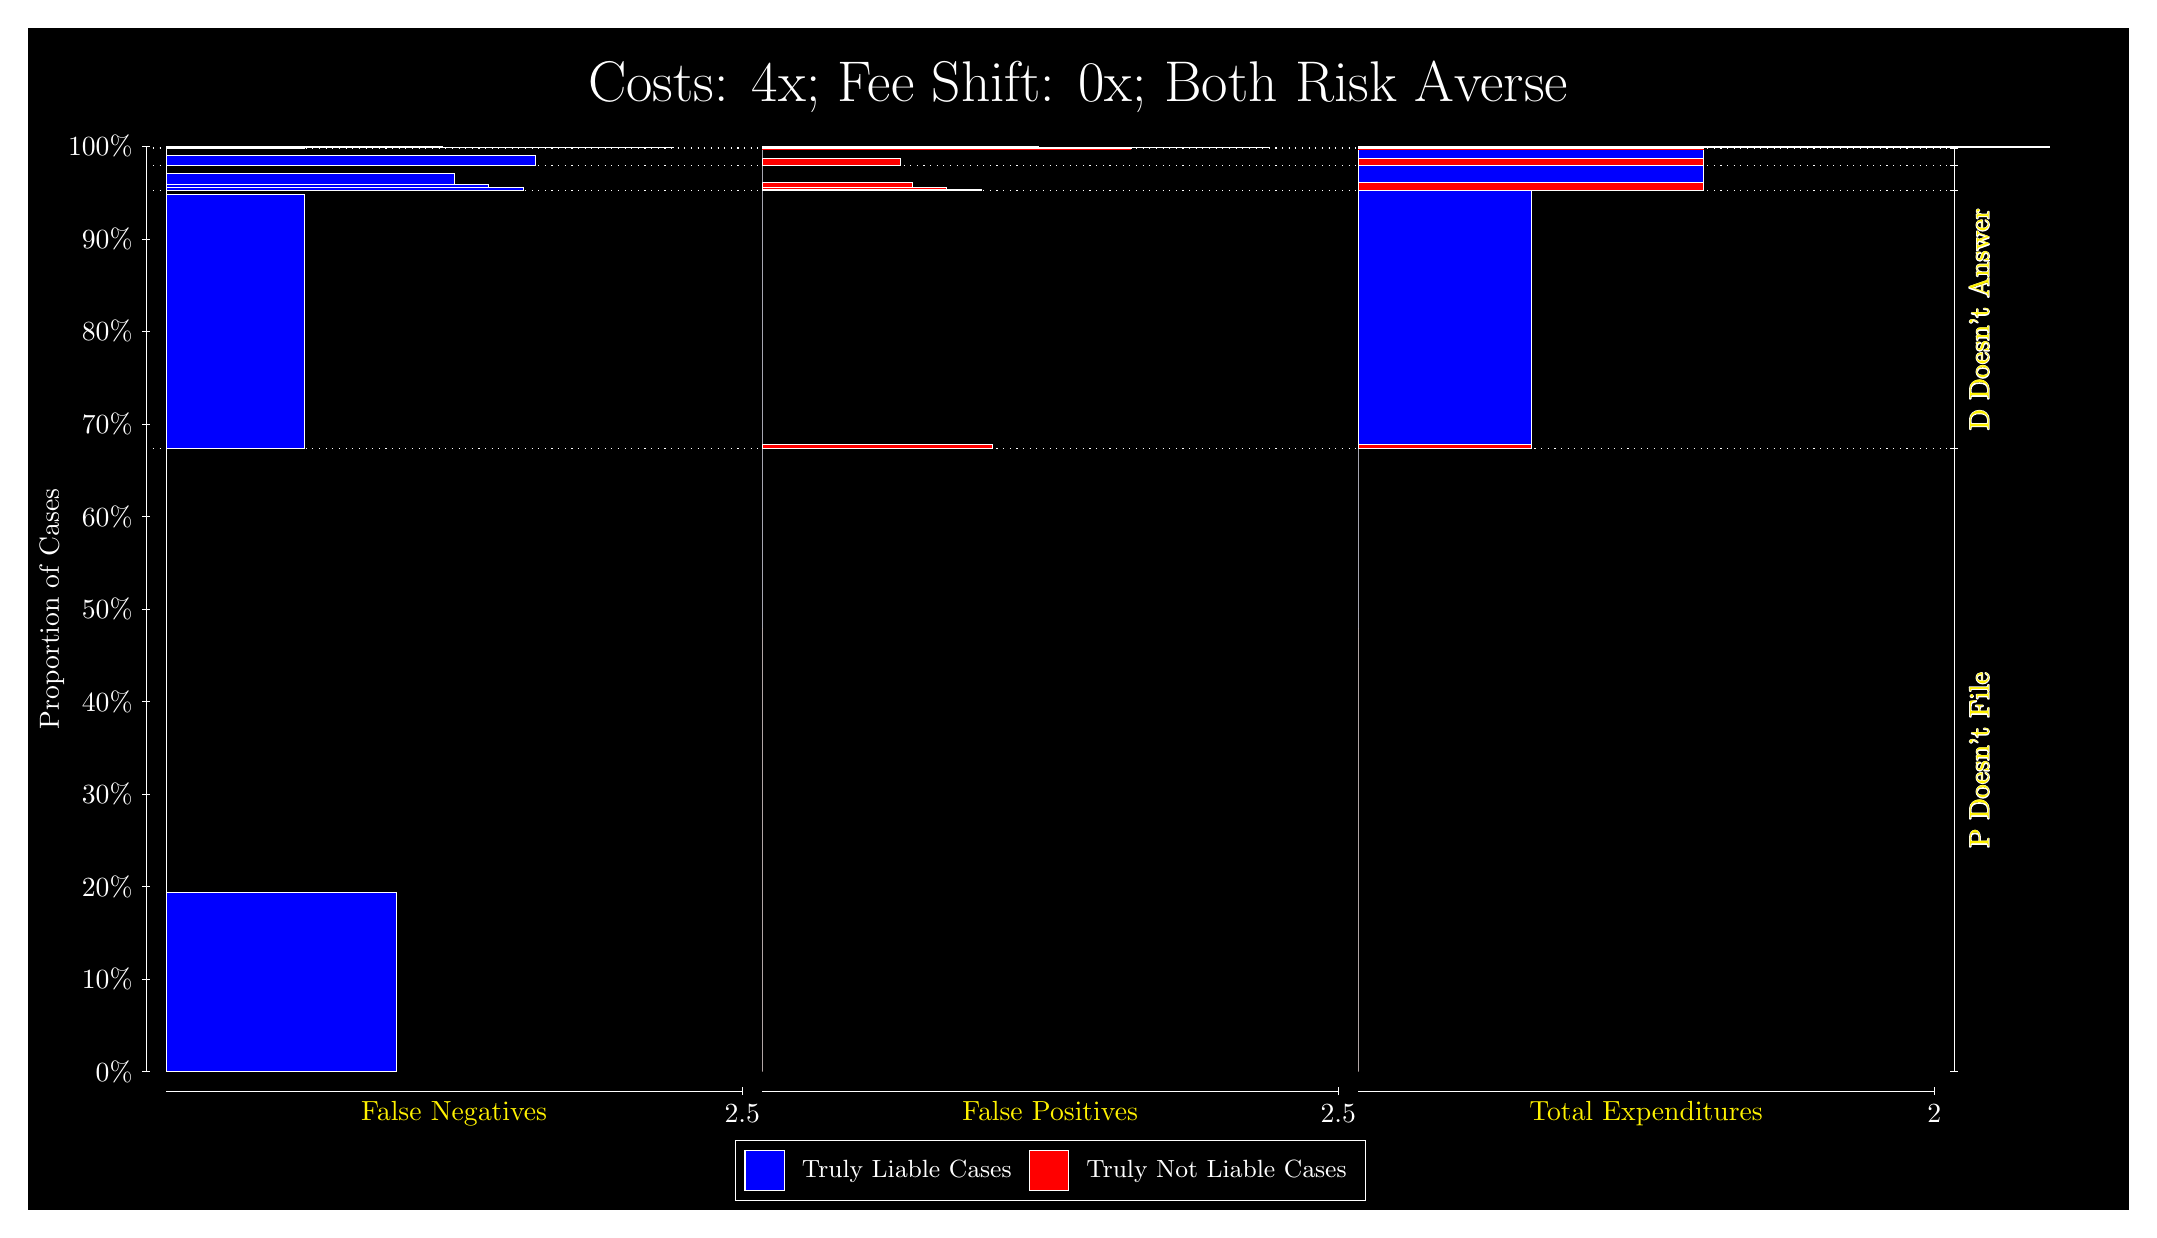
\begin{tikzpicture}
\draw[fill=black] (0,0) rectangle (26.667,15);
\draw[text=white] (0,13.5) rectangle (26.667,15) node[midway] {\huge Costs: 4x; Fee Shift: 0x; Both Risk Averse};
\draw[white, very thin] (1.5,1.75) -- (1.5,13.5);
\node[rotate=90, text=white, anchor=center] at (0.3, 7.625) {Proportion of Cases};
\draw[white, very thin] (1.45,1.75) -- (1.55,1.75);
\node[text=white, anchor=east] at (1.45, 1.75) {0\%};
\draw[white, very thin] (1.45,2.925) -- (1.55,2.925);
\node[text=white, anchor=east] at (1.45, 2.925) {10\%};
\draw[white, very thin] (1.45,4.1) -- (1.55,4.1);
\node[text=white, anchor=east] at (1.45, 4.1) {20\%};
\draw[white, very thin] (1.45,5.275) -- (1.55,5.275);
\node[text=white, anchor=east] at (1.45, 5.275) {30\%};
\draw[white, very thin] (1.45,6.45) -- (1.55,6.45);
\node[text=white, anchor=east] at (1.45, 6.45) {40\%};
\draw[white, very thin] (1.45,7.625) -- (1.55,7.625);
\node[text=white, anchor=east] at (1.45, 7.625) {50\%};
\draw[white, very thin] (1.45,8.8) -- (1.55,8.8);
\node[text=white, anchor=east] at (1.45, 8.8) {60\%};
\draw[white, very thin] (1.45,9.975) -- (1.55,9.975);
\node[text=white, anchor=east] at (1.45, 9.975) {70\%};
\draw[white, very thin] (1.45,11.15) -- (1.55,11.15);
\node[text=white, anchor=east] at (1.45, 11.15) {80\%};
\draw[white, very thin] (1.45,12.325) -- (1.55,12.325);
\node[text=white, anchor=east] at (1.45, 12.325) {90\%};
\draw[white, very thin] (1.45,13.5) -- (1.55,13.5);
\node[text=white, anchor=east] at (1.45, 13.5) {100\%};

\draw[white, very thin] (24.457,1.75) -- (24.457,13.5);
\draw[white, very thin] (24.407,1.75) -- (24.507,1.75);
\node[anchor=west] at (24.407, 1.75) {};
\draw[white, very thin] (24.407,9.6649) -- (24.507,9.6649);
\node[anchor=west] at (24.407, 9.6649) {};
\draw[white, very thin] (24.407,12.941) -- (24.507,12.941);
\node[anchor=west] at (24.407, 12.941) {};
\draw[white, very thin] (24.407,13.259) -- (24.507,13.259);
\node[anchor=west] at (24.407, 13.259) {};
\draw[white, very thin] (24.407,13.471) -- (24.507,13.471);
\node[anchor=west] at (24.407, 13.471) {};
\draw[white, very thin] (24.407,13.484) -- (24.507,13.484);
\node[anchor=west] at (24.407, 13.484) {};
\draw[white, very thin] (24.407,13.489) -- (24.507,13.489);
\node[anchor=west] at (24.407, 13.489) {};
\draw[white, very thin] (24.407,13.5) -- (24.507,13.5);
\node[anchor=west] at (24.407, 13.5) {};

\draw[white, very thin, fill=blue] (1.75,1.75) rectangle (4.6775,4.0326);
\draw[white, very thin, fill=red] (1.75,4.0326) rectangle (1.75,9.6649);
\draw[white, very thin, fill=blue] (1.75,9.6649) rectangle (3.5065,12.888);
\draw[white, very thin, fill=red] (1.75,12.888) rectangle (1.75,12.941);
\draw[white, very thin, fill=blue] (1.75,12.941) rectangle (6.2877,12.979);
\draw[white, very thin, fill=blue] (1.75,12.979) rectangle (5.8486,13.021);
\draw[white, very thin, fill=blue] (1.75,13.021) rectangle (5.4094,13.16);
\draw[white, very thin, fill=red] (1.75,13.16) rectangle (1.75,13.259);
\draw[white, very thin, fill=blue] (1.75,13.259) rectangle (6.4341,13.385);
\draw[white, very thin, fill=red] (1.75,13.385) rectangle (1.75,13.471);
\draw[white, very thin, fill=blue] (1.75,13.471) rectangle (3.5065,13.484);
\draw[white, very thin, fill=red] (1.75,13.484) rectangle (1.75,13.484);
\draw[white, very thin, fill=blue] (1.75,13.484) rectangle (8.1906,13.486);
\draw[white, very thin, fill=red] (1.75,13.486) rectangle (1.75,13.489);
\draw[white, very thin, fill=blue] (1.75,13.489) rectangle (5.2631,13.5);
\draw[white, very thin, fill=red] (1.75,13.5) rectangle (1.75,13.5);
\draw[white, very thin, fill=red] (9.3189,1.75) rectangle (9.3189,7.3823);
\draw[white, very thin, fill=blue] (9.3189,7.3823) rectangle (9.3189,9.6649);
\draw[white, very thin, fill=red] (9.3189,9.6649) rectangle (12.246,9.718);
\draw[white, very thin, fill=blue] (9.3189,9.718) rectangle (9.3189,12.941);
\draw[white, very thin, fill=red] (9.3189,12.941) rectangle (12.1,12.96);
\draw[white, very thin, fill=red] (9.3189,12.96) rectangle (11.661,12.975);
\draw[white, very thin, fill=red] (9.3189,12.975) rectangle (11.222,13.04);
\draw[white, very thin, fill=blue] (9.3189,13.04) rectangle (9.3189,13.259);
\draw[white, very thin, fill=red] (9.3189,13.259) rectangle (11.075,13.344);
\draw[white, very thin, fill=blue] (9.3189,13.344) rectangle (9.3189,13.471);
\draw[white, very thin, fill=red] (9.3189,13.471) rectangle (14.003,13.472);
\draw[white, very thin, fill=blue] (9.3189,13.472) rectangle (11.075,13.484);
\draw[white, very thin, fill=red] (9.3189,13.484) rectangle (12.832,13.488);
\draw[white, very thin, fill=blue] (9.3189,13.488) rectangle (9.9044,13.489);
\draw[white, very thin, fill=red] (9.3189,13.489) rectangle (15.759,13.49);
\draw[white, very thin, fill=blue] (9.3189,13.49) rectangle (12.832,13.5);
\draw[white, very thin, fill=red] (16.888,1.75) rectangle (16.888,7.3823);
\draw[white, very thin, fill=blue] (16.888,7.3823) rectangle (16.888,9.6649);
\draw[white, very thin, fill=red] (16.888,9.6649) rectangle (19.083,9.718);
\draw[white, very thin, fill=blue] (16.888,9.718) rectangle (19.083,12.941);
\draw[white, very thin, fill=red] (16.888,12.941) rectangle (21.279,13.04);
\draw[white, very thin, fill=blue] (16.888,13.04) rectangle (21.279,13.259);
\draw[white, very thin, fill=red] (16.888,13.259) rectangle (21.279,13.344);
\draw[white, very thin, fill=blue] (16.888,13.344) rectangle (21.279,13.471);
\draw[white, very thin, fill=red] (16.888,13.471) rectangle (21.279,13.472);
\draw[white, very thin, fill=blue] (16.888,13.472) rectangle (21.279,13.484);
\draw[white, very thin, fill=red] (16.888,13.484) rectangle (25.67,13.488);
\draw[white, very thin, fill=blue] (16.888,13.488) rectangle (25.67,13.489);
\draw[white, very thin, fill=red] (16.888,13.489) rectangle (25.67,13.49);
\draw[white, very thin, fill=blue] (16.888,13.49) rectangle (25.67,13.5);
\draw[white, dotted] (1.5,9.6649) -- (24.457,9.6649);
\draw[white, dotted] (1.5,12.941) -- (24.457,12.941);
\draw[white, dotted] (1.5,13.259) -- (24.457,13.259);
\draw[white, dotted] (1.5,13.471) -- (24.457,13.471);
\draw[white, dotted] (1.5,13.484) -- (24.457,13.484);
\draw[white, dotted] (1.5,13.489) -- (24.457,13.489);
\draw[white, very thin] (1.75,1.5) -- (9.0689,1.5);
\node[text=yellow, anchor=north] at (5.4094, 1.5) {False Negatives};
\draw[white, very thin] (9.0689,1.45) -- (9.0689,1.55);
\node[text=white, anchor=north] at (9.0689, 1.45) {2.5};

\draw[white, very thin] (9.3189,1.5) -- (16.638,1.5);
\node[text=yellow, anchor=north] at (12.978, 1.5) {False Positives};
\draw[white, very thin] (16.638,1.45) -- (16.638,1.55);
\node[text=white, anchor=north] at (16.638, 1.45) {2.5};

\draw[white, very thin] (16.888,1.5) -- (24.207,1.5);
\node[text=yellow, anchor=north] at (20.547, 1.5) {Total Expenditures};
\draw[white, very thin] (24.207,1.45) -- (24.207,1.55);
\node[text=white, anchor=north] at (24.207, 1.45) {2};

\node[text=yellow, centered, rotate=90] at (24.777, 5.7075) {\contour{white}{P Doesn't File}};
\node[text=yellow, centered, rotate=90] at (24.777, 11.303) {\contour{white}{D Doesn't Answer}};






\draw (12.978300999999998,1.5) node[draw=none] (baseCoordinate) {};
\begin{scope}[align=center]
        \matrix[scale=0.5, draw=white, below=0.5cm of baseCoordinate, nodes={draw}, column sep=0.1cm]{
            \node[rectangle, draw, minimum width=0.5cm, minimum height=0.5cm, fill=blue] {}; &
            \node[draw=none, font=\small, text=white] (B) {Truly Liable Cases}; &
            \node[rectangle, draw, minimum width=0.5cm, minimum height=0.5cm, fill=red] {}; &
            \node[draw=none, font=\small, text=white] (B) {Truly Not Liable Cases}; \\
            };
\end{scope}

\end{tikzpicture}
\end{document}